\chapter{Verificações, validações e análises}\label{Algumas_verificacoes_validacoes}

\section{Validação referente ao endurecimento e amolecimento da parte elastoplástica através de um ensaio}

Uma vez que se tem um ensaio triaxial, como por exemplo, o da \autoref{ensaio_triaxial_ductil} uma validação do endurecimento e amolecimento da parte elastoplástica é possível. Os modelos estão apresentados na \autoref{malha_ensaio_triaxial} e compreendem a simulação numérica de um ensaio considerando um modelo 3D, estado plano de deformação e axissimétrico. Sendo $l_a = l_b = l_c = 1$ o próprio deslocamento em y do nó A será a deformação específica. Para representar o ensaio da \autoref{ensaio_triaxial_ductil} foi aplicado um deslocamento imposto $\delta = 0.1$ na face superior.

\begin{figure}[H]
	\begin{center}
		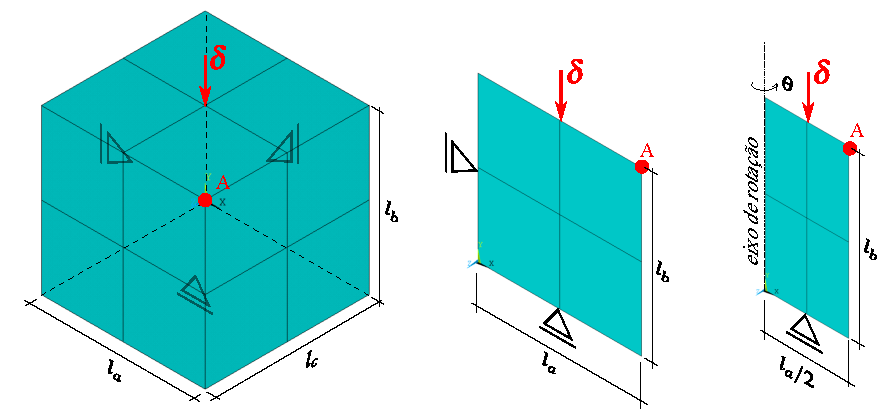
\includegraphics[scale = 1.0]{0701-Malha_ensaio_triaxial.pdf}
	\end{center}
	\caption{\label{malha_ensaio_triaxial}Domínio e discretização de um ensaio triaxial com modelo 3D, EPD e AXI}
\end{figure}

Os valores dos parâmetros do modelo constitutivo adotado na análise foram $E = 403$MPa, $\nu = 0.39$,  superficief = 2, superficieg = 2, $\phi = 0, \psi = 0, c_i = 0,7, c_p = 1,3, c_r = 0,9, \bar \varepsilon^p_{I} = 0,010, \bar \varepsilon^p_{II} = 0,050, \bar \varepsilon^p_{r} = 0,07$, Dalg = 0. Os parâmetros de coesão e de deformação plástica equivalente das zonas de endurecimento e amolecimento são coletadas do gráfico do ensaio, tal como apresentado na \autoref{ensaio_triaxial_parametros}. O valor de duas vezes a coesão está no fato de que não está sendo considerado o ângulo de atrito e de dilatância, fazendo com que a superfície de plasticidade se reduza a de von-Mises. Nesse aspecto, a variação do volume não considera a dilatância durante a deformação plástica. A parte viscosa do modelo constitutivo é eliminada utilizando uma coesão alta. O resultado da análise pode ser visto na \autoref{ensaio_triaxial_solucao}.
 
\begin{figure}[H]
 	\begin{center}
 		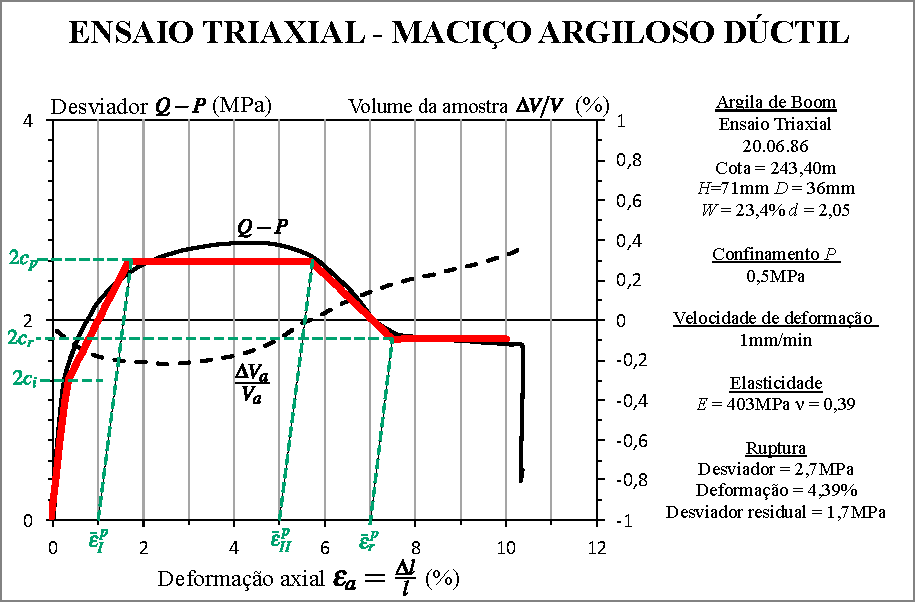
\includegraphics[scale = 0.9]{0702-ensaio triaxial argila ductil_coletando_parametros.pdf}
 	\end{center}
 	\caption{\label{ensaio_triaxial_parametros}Domínio e discretização de um ensaio triaxial com modelo 3D, EPD e AXI}
\end{figure}

\begin{figure}[H]
	\begin{center}
		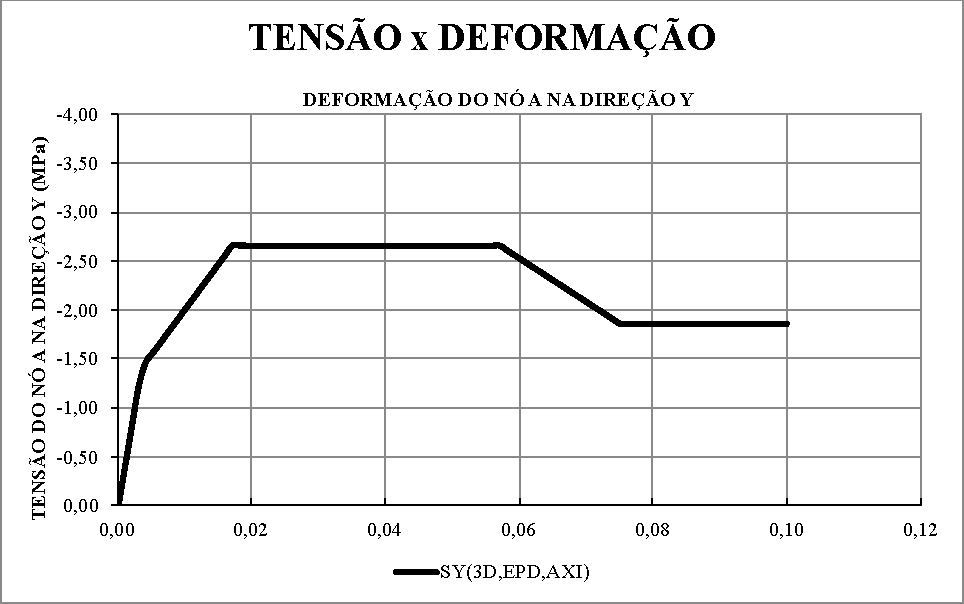
\includegraphics[scale = 1.0]{0703-ensaio triaxial argila ductil solucao.pdf}
	\end{center}
	\caption{\label{ensaio_triaxial_solucao}Resultado da análise para o ensaio triaxial}
\end{figure}

Como pode-se ver os valores deram exatamente iguais considerando 3D, EPD e AXI demonstrando que a implementação conseguiu essa generalidade. Caso o modelo seja de fato utilizado para estudos de túneis reais é sempre desejável ter ensaios triaxiais para fazer a validação ou eventuais calibrações nesse aspecto do modelo.

\section{Verificação da solução numérica com uma solução analítica considerando o endurecimento}

Essa verificação considerará uma das soluções analíticas deduzidas por \citeonline{Bernaud2020}. A solução analítica escolhida corresponde a um problema de um túnel profundo de seção circular sobre tensão geostática hidrostática com um critério de plasticidade de Tresca considerando endurecimento por deformação plástica, conforme \autoref{coesao_solucao_analitca_LAJSS}. 

\begin{figure}[H]
	\begin{center}
		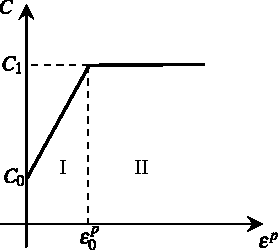
\includegraphics[scale = 1.2]{0704-lei de endurecimento ou amolecimento_coesao_solucao_analitca.pdf}
	\end{center}
	\caption{\label{coesao_solucao_analitca_LAJSS}Variação da coesão: I - trecho de endurecimento linear e II - comportamento perfeitamente plástico (adaptado de: \citeonline[p.  4]{Bernaud2020})}
\end{figure}
A expressão (\ref{eq:LAJSS1}) apresenta a solução analítica da convergência quando se adota $r=R_i$.
\begin{equation}
	\label{eq:LAJSS1}
	\dfrac{u(r)}{r} = \dfrac{(1-2\nu)(\nu+1)}{E}\left\{\sigma_x+\dfrac{2C_0}{1+2\dfrac{C'}{E'}}\left[\dfrac{C'}{E'}\left(\dfrac{1}{r^2}-\dfrac{1}{x^2}\right) y^2+\ln{\left(\dfrac{x}{r}\right)-\sigma_\infty} \right]  \right\}-\dfrac{2C_0}{E'}\left(\dfrac{y}{r}\right)^2
\end{equation}
em que $E'=E/(1+\nu), \nu, C' = (C_1-C_0)/\varepsilon_0^p$ são parâmetros do material. Essa solução é dependente também dos raios plásticos $x,~y$, da tensão na fronteira do raio plástico $\sigma_x$, das tensões geostáticas hidrostáticas $\sigma_\infty$ e da tensão no interior da cavidade do túnel $\sigma_i$. O restante das expressões para aplicar essa solução são:
\begin{equation} \label{eq:LAJSS2}
	{{\sigma }_{x}}=2{{C}_{1}}\ln \left( \frac{{{R}_{i}}}{x} \right)+{{\sigma }_{i}},~~~ 	{{x}^{2}}=\frac{2{{C}_{0}}}{E'\varepsilon _{0}^{p}+2{{C}_{1}}}{{y}^{2}}, ~~~ 	{{y}^{2}}=\frac{{{R}_{i}}}{{{\omega }_{0}}}{{e}^{\frac{({{\omega }_{1}}+{{\omega }_{2}}+{{\omega }_{3}})}{{{C}_{1}}}}} 
\end{equation}
\begin{equation} \label{eq:LAJSS3}
	{{\omega }_{0}}=\frac{2{{C}_{0}}}{E'\varepsilon _{0}^{p}+2{{C}_{1}}}, ~~~ 	{{\omega }_{1}}={{\sigma }_{i}}-{{\sigma }_{\infty }}-{{C}_{0}} , ~~~ {{\omega }_{2}}=\frac{{{C}_{0}}}{1+2\frac{C'}{E'}}\ln ({{\omega }_{0}}), ~~~ 	{{\omega }_{3}}=\frac{\frac{C'}{E'}\left[ 2({{C}_{0}}-{{C}_{1}})-\varepsilon _{0}^{p} \right]}{1+2\frac{C'}{E'}}
\end{equation}

Utilizando $Ri=1$m, $E=1430$MPa, $\nu = 0.4$, $C_0=0.21$MPa, $C_1=0.56$MPa, $\varepsilon _{0}^{p}=0.024$, $P_i = -\sigma_i = 2.5$MPa, $ P_\infty = -\sigma_\infty = 4.5$MPa tem-se, pela expressão analítica, $U_i(\%) = 5.91$. A Figura \autoref{solucao_numérica_LAJSS} apresenta a concordância do resultado numérico com um erro menor que 1\%.

\begin{figure}[H]
	\begin{center}
		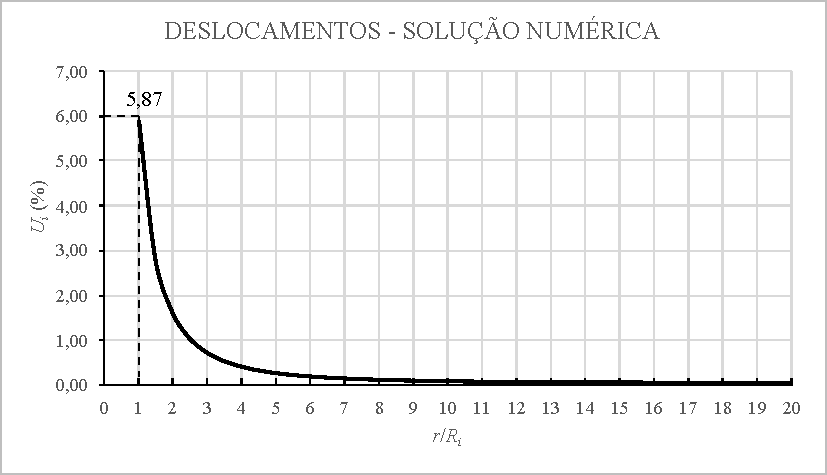
\includegraphics[scale = 1.0]{0705-lei de endurecimento ou amolecimento_coesao_solucao_numerica.pdf}
	\end{center}
	\caption{\label{solucao_numérica_LAJSS}Solução numérica considerando elastoplasticidade com endurecimento}
\end{figure}
Para essa solução numérica foi utilizado domínio em EPD (\autoref{malhaEPD_tunel}) e a relação (\ref{eq:ctr_cvm}) que considera a superfície de von-Mises inscrita em Tresca e as mesmas considerações para particularizar o modelo elastoplástico-viscoplástico para elastoplástico, ou seja, a parte viscosa do modelo constitutivo é novamente eliminada utilizando uma coesão viscosa alta. Para representar a mesma lei de endurecimento tem-se $c_i = 0.21\sqrt{3}/2$, $c_p = 0.56\sqrt{3}/2$, $c_r = 0.56\sqrt{3}/2, \bar \varepsilon^p_{I} = 0,024, \bar \varepsilon^p_{II} = 0,024, \bar \varepsilon^p_{r} = 0,024$. 

\section{Verificação do modelo acoplado com cada comportamento em separado}
O modelo constitutivo elastoplástico-viscoplástico é bastante geral e capaz de reproduzir cada comportamento em seperado. Portanto, é apresentado algumas verificações da solução numérica considerando cada lei constitutiva separada: I - elasticidade, II - elastoplasticidade e III - viscoplasticidade. Para o caso I e II sem revestimento é utilizado soluções analíticas como comparação. A expressão dessas podem ser encontradas em \citeonline{Corbeta1990} e \citeonline[p. 50-54]{Quevedo2017} e portanto não serão apresentadas. A solução elastoplástica considera uma plasticidade perfeita com regra de fluxo associada com superfície de escoamento de Tresca. Para outros casos e quando se tem revestimento a verificação foi feita com outro \textit{software}, o GEOMEC91. O GEOMEC91 é um programa de elementos finitos para geomecânica para análises bidimensionais em axissimetria. Ele foi desenvolvido por \citeonline{Bernaud1991} e detalhes de sua malha e condições de contorno podem ser vistas em \citeonline[p. 190]{Bernaud1991}.

Os resultados apresentados nessa seção são os obtidos do modelo axissimétrico da \autoref{malhaAXI_tunel} com os parâmetros da \autoref{parametros_AXI}. Apesar de estar limitado às condições de axissimetria, é um dos modelos mais importantes, pois considera o processo de escavação e colocação do revestimento de forma realista e permite fazer estudos paramétricos de forma mais eficiente que os modelos tridimensionais. Contudo, as mesmas verificações foram feitas no modelo tridimensional considerando seção circular e os mesmos resultados foram obtidos, com pequenas diferenças menores que 1\%.

\subsection{Verificações em elasticidade}

O modelo constitutivo acoplado, por ser geral, tem que ser capaz de reproduzir o resultado em elasticidade colocando coesões elevadas na parte plástica e viscosa. Dessa forma, considerando $E =$1000MPa e 5000MPa, $\nu =$ 0.498MPa, $p_v = p_h = 5$MPa tem-se os resultados da \autoref{ELAST-D0-E1000-ER0-P5} e \autoref{ELAST-D0-E5000-ER0-P5}. As curvas cinzas são os perfis de convergência a cada passo de escavação e a vermelha no último passo. A curva verde pontilhada é a solução analítica.

\begin{figure}[H]
	\begin{center}
		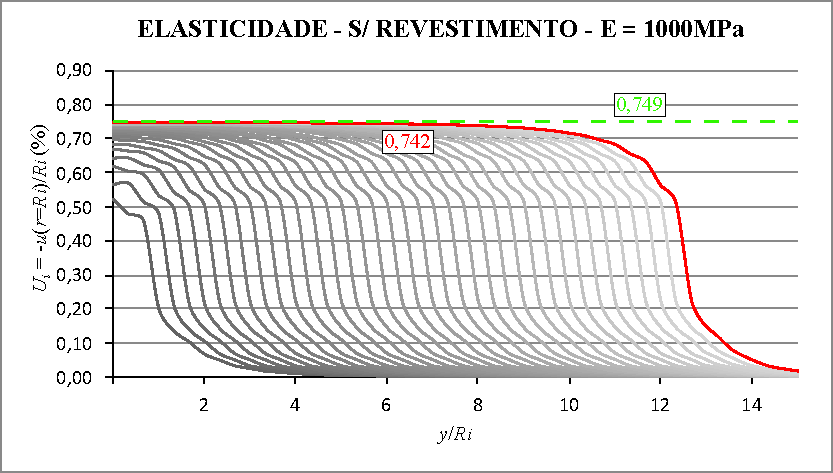
\includegraphics[scale = 1.0]{0706-AXI-SREVESTIMENTO-E1000.pdf}
	\end{center}
	\caption{\label{ELAST-D0-E1000-ER0-P5}Verificação solução numérica em elasticidade sem revestimento - E = 1000MPa}
\end{figure}

\begin{figure}[H]
	\begin{center}
		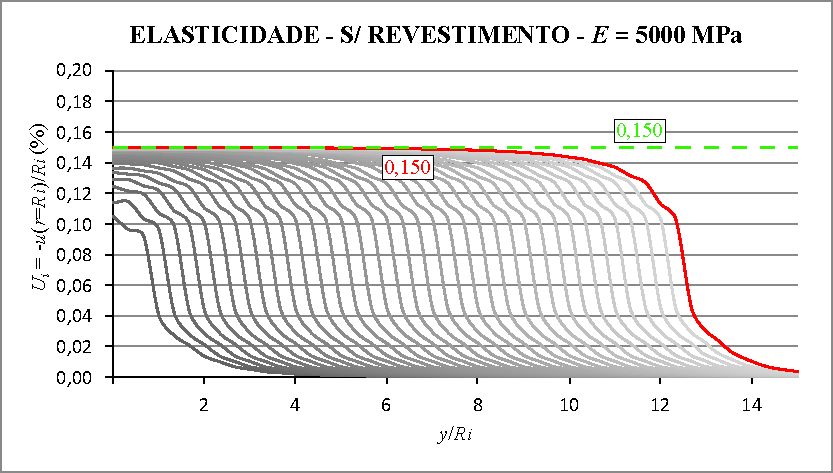
\includegraphics[scale = 1.0]{0707-AXI-SREVESTIMENTO-E5000.pdf}
	\end{center}
	\caption{\label{ELAST-D0-E5000-ER0-P5}Verificação solução numérica em elasticidade sem revestimento - E = 5000MPa}
\end{figure}

Cabe salientar que em elasticidade a mesma solução é obtida escavando todos os passos de uma única vez. Contudo, quando se tem revestimento não há solução analítica, pois ocorre a iteração entre o revestimento e o maciço. Para essa verificação é comparado o resultado do ANSYS com o GEOMEC91. A \autoref{ELAST-D0-E1000-ER30000-P5} mostra essa comparação considerando $E$ = 1000MPa com um revestimento de $E_{rev}$=30000MPa e $\nu_{rev}$ = 0,3. Nesse caso, foi considerado um $d0$ = 0.

\begin{figure}[H]
	\begin{center}
		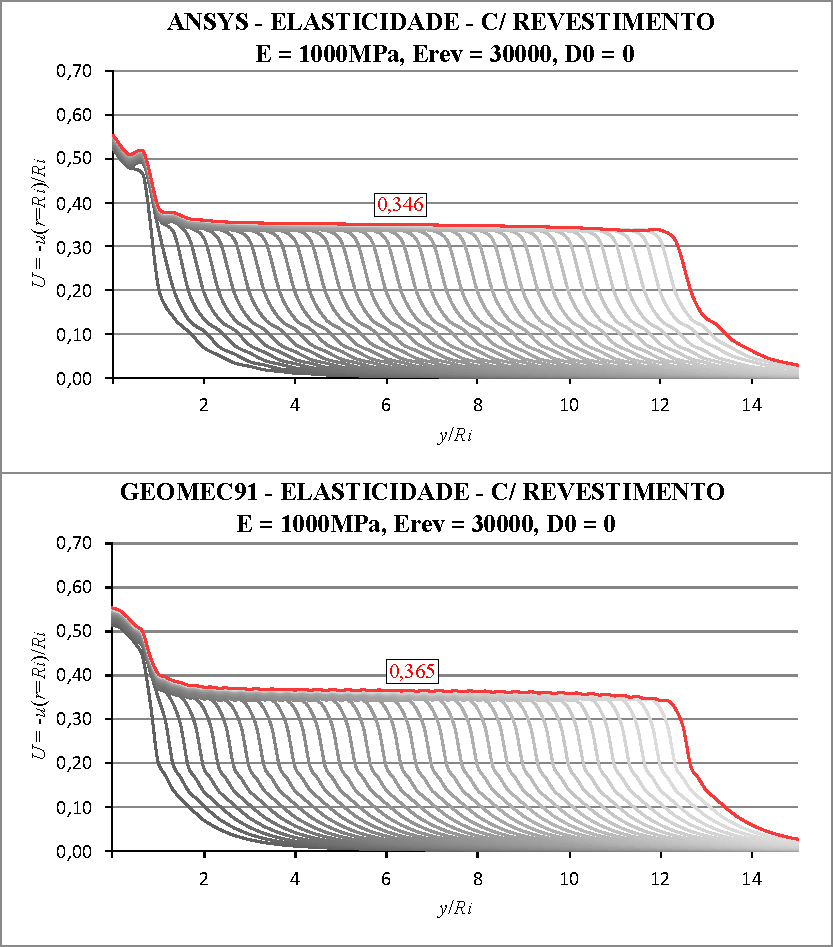
\includegraphics[scale = 1.0]{0708-AXI-SREVESTIMENTO-E1000-ER30000-D0.pdf}
	\end{center}
	\caption{\label{ELAST-D0-E1000-ER30000-P5}Verificação solução numérica em elasticidade com revestimento - $E$ = 1000MPa, $E_{rev}$ = 30000MPa, $d0$ = 0}
\end{figure}

O perfil de convergência apresenta um pico nas primeiras escavações, uma vez que na primeira escavação é escavado 3$L_p$. De qualquer forma, em comparação com a \autoref{ELAST-D0-E1000-ER0-P5} consegue-se ver que o revestimento tem um grande efeito sobre as deformações. Contudo, não é só o módulo de elasticidade do revestimento que conta, mas tão importante quanto, o d0. Considerando um $d_0=4L_p$ tem-se os resultados da \autoref{ELAST-D4-E1000-ER30000-P5}.

\begin{figure}[H]
	\begin{center}
		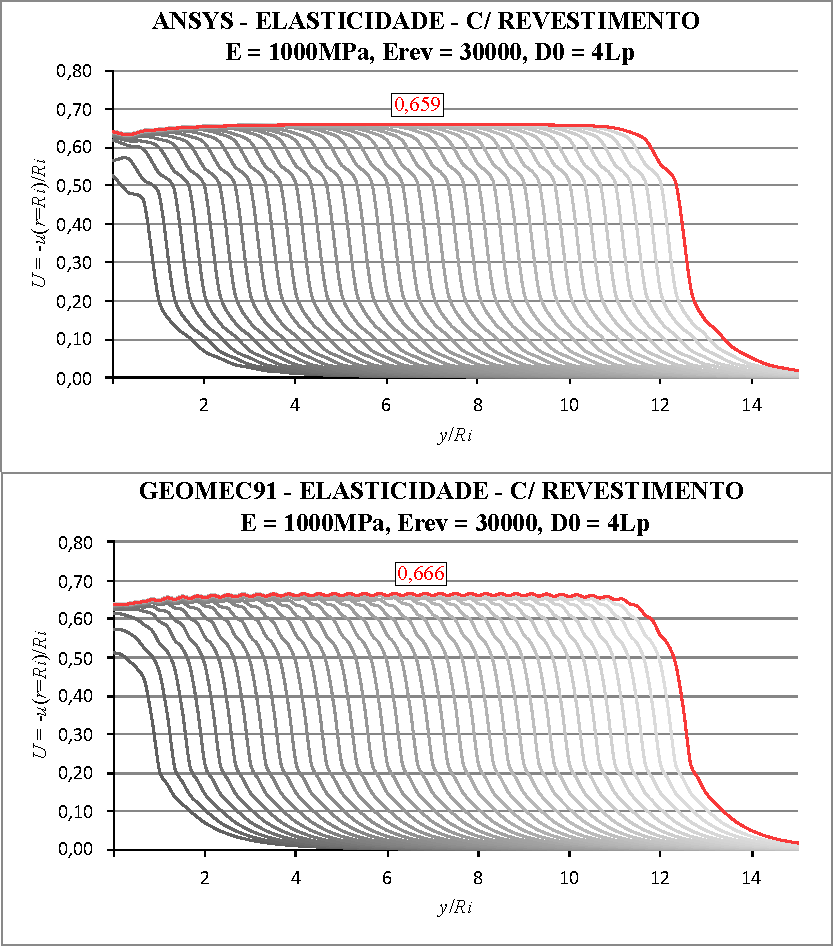
\includegraphics[scale = 1.0]{0709-AXI-SREVESTIMENTO-E1000-ER30000-D4.pdf}
	\end{center}
	\caption{\label{ELAST-D4-E1000-ER30000-P5}Verificação solução numérica em elasticidade com revestimento - $E$ = 1000MPa, $E_{rev}$ = 30000MPa, $d0$ = 4$L_p$}
\end{figure}

Na \autoref{ELAST-D4-E1000-ER30000-P5} pode-se ver pequenas ondulações no perfil de convergências do GEOMEC91 que não estão presentes no resultado do ANSYS. Essa diferença ocorre devido ao elemento finito utilizado. No GEOMEC91 é utilizado um elmento quadrático enquanto que no ANSYS linear.

Como pode-se notar o modelo constitutivo acoplado conseguiu em elasticidade reproduzir outras soluções independentes. Ademais, a verificação do modelo em elasticidade é muito importante para conferir se as escavações e a colocação do revestimento estavam sendo feitas corretamente. Além disso, deram uma ideia inicial da qualidade da malha.

\subsection{Verificações em elastoplasticidade}

De forma análoga à elasticidade, o modelo constitutivo acoplado, por ser geral, tem que ser capaz de reproduzir o resultado em elastoplasticidade colocando uma coesão viscoplástica elevada. Considerando $E =$1000MPa, $\nu =$ 0.498MPa, $p_v = p_h = 4$MPa, $c_i=c_p=c_r = \sqrt{3}/2$MPa e $3\sqrt{3}/2$MPa  tem-se os resultados da \autoref{PLAST-D0-E1000-ER0-P4-C1} e \autoref{PLAST-D0-E1000-ER0-P4-C3}. As curvas cinzas são os perfis de convergência a cada passo de escavação e a vermelha no último passo. A curva verde pontilhada é a solução analítica.

\begin{figure}[H]
	\begin{center}
		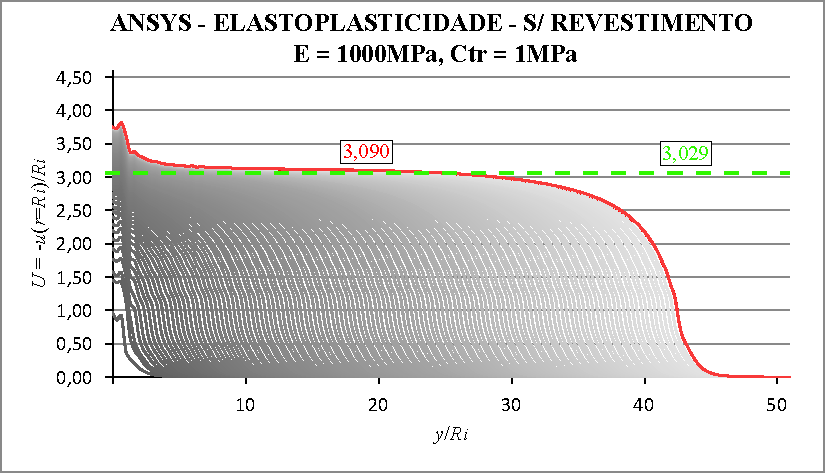
\includegraphics[scale = 1.0]{0710-AXI-PLAST-SREVESTIMENTO-D0-E1000-ER0-P4-C1.pdf}
	\end{center}
	\caption{\label{PLAST-D0-E1000-ER0-P4-C1}Verificação solução numérica em elasticidade com revestimento - $E$ = 1000MPa,  $c_i=c_p=c_r = \sqrt{3}/2$MPa}
\end{figure}
No caso em que $c_i=c_p=c_r = \sqrt{3}/2$MPa, foi necessário aumentar o número de passos de escavação $n_p = 128$ para que o patamar no perfil de convergência se desenvolvesse plenamente. A solução analítica é dada para esse patamar sem a influência da face de escavação ou das bordas do modelo. Isso mostra que dependendo dos valores dos parâmetros a malha tem que sofrer ajustes. Se o valor almejado é a convergência no equilíbrio fora das zonas de influência deve-se buscar uma malha suficiente para aparecer o patamar no perfil de convergências. Um outro aspecto em que a malha muitas vezes deve ser ajustada é quando as deformações plásticas alcançam as bordas do domínio, sendo nesse caso necessário aumentar o limites do domínio ($L_x, L_y$ e $L_z$). Para o domínio escolhido resultados são obtidos de forma satisfatória sempre que a relação da pressão geostática-hidrostática pela coesão for menor ou igual a 5.
\begin{figure}[H]
	\begin{center}
		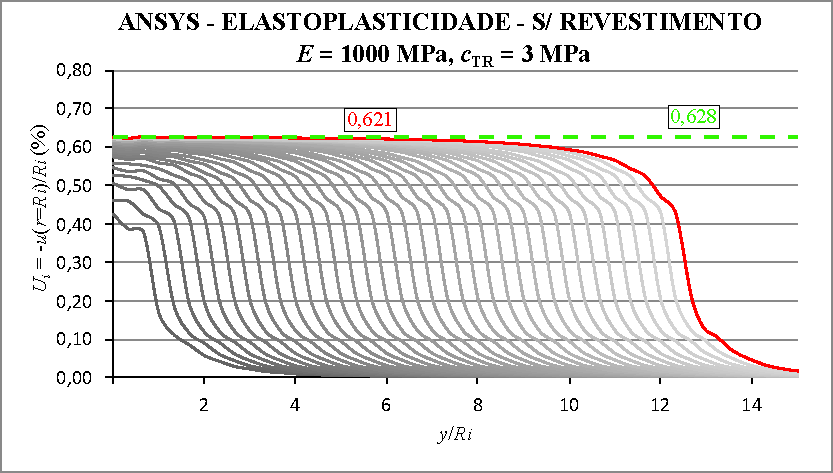
\includegraphics[scale = 1]{0711-AXI-PLAST-SREVESTIMENTO-D0-E1000-ER0-P4-C3.pdf}
	\end{center}
	\caption{\label{PLAST-D0-E1000-ER0-P4-C3}Verificação solução numérica em elasticidade com revestimento - $E$ = 1000MPa, $c_i=c_p=c_r = 3\sqrt{3}/2$MPa}
\end{figure}
 A próxima verificação, compreende a plasticidade dependente da pressão e não associada. Para tanto é utilizado um ângulo de atrito $\phi$=15$^\circ$ e um ângulo de dilatância $\psi$=0$^\circ$. O resultado pode ser visto na \autoref{PLAST-D0-E1000-ER0-P4-C1-KP15-KB1}. Essa solução apenas não converge quando se utiliza Newton-Raphson Completo com o módulo constitutivo consistente. Se for utilizar o módulo constitutivo consistente é necessário utilizar o Newton-Raphson Completo Assimétrico. A opção em que é utilizado Newton-Raphson Completo mas sem atualizar o módulo constitutivo converge para a solução. Outro aspecto importante, comparando o resultado da \autoref{PLAST-D0-E1000-ER0-P4-C1-KP15-KB1} com a \autoref{PLAST-D0-E1000-ER0-P4-C1} é a sensibilidade com que a convergência é afetada pelo ângulo de atrito. Esse resultado é esperado uma vez que quanto maior o ângulo de atrito, para uma dada pressão hidrostática, mais afastado fica a superfície de plastificação do eixo hidrostático.
\begin{figure}[H]
	\begin{center}
		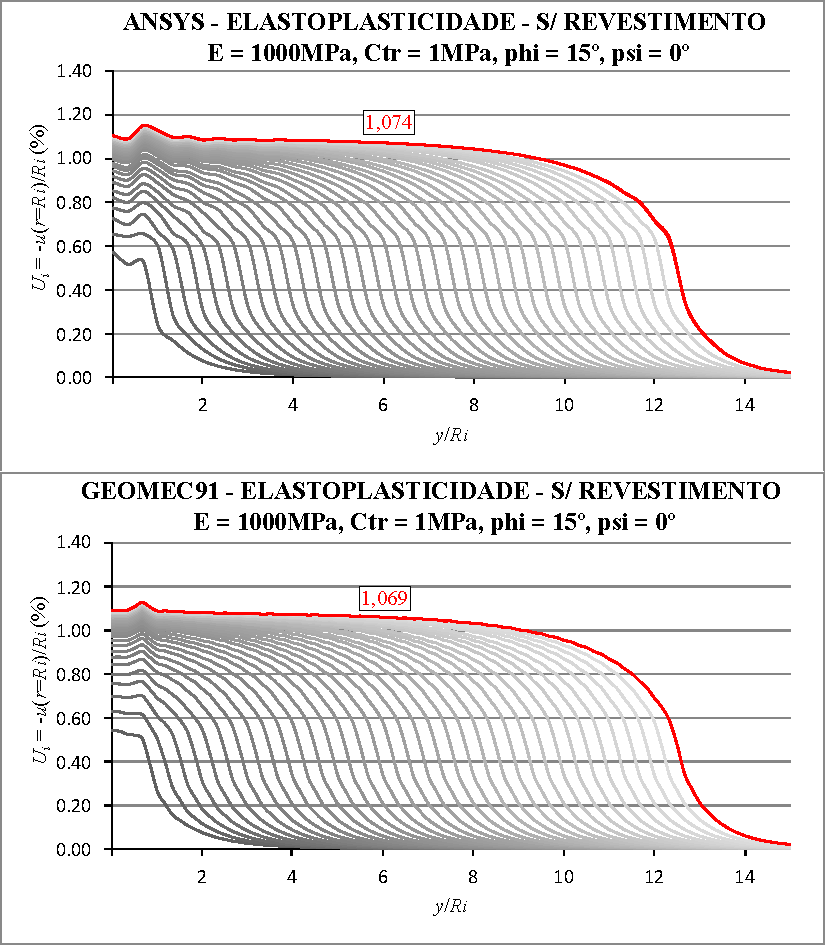
\includegraphics[scale = 1]{0712-AXI-PLAST--D0-E1000-ER0-P4-C1-KP15-KB1.pdf}
	\end{center}
	\caption{\label{PLAST-D0-E1000-ER0-P4-C1-KP15-KB1}Verificação solução numérica elastoplasticidade sem revestimento $E$ = 1000MPa, $c_i=c_p=c_r = \sqrt{3}/2$MPa, $\phi$=15$^\circ$ e $\psi$=0$^\circ$}
\end{figure}

A verificação da solução considerando a colocação de um revestimento com $E_{rev} = 30000$MPa, $\nu_{rev} = 0,3$ e $d_0=0$ pode ser vista na \ref{PLAST-D0-E1000-ER30000-P4-C1}.

\begin{figure}[H]
	\begin{center}
		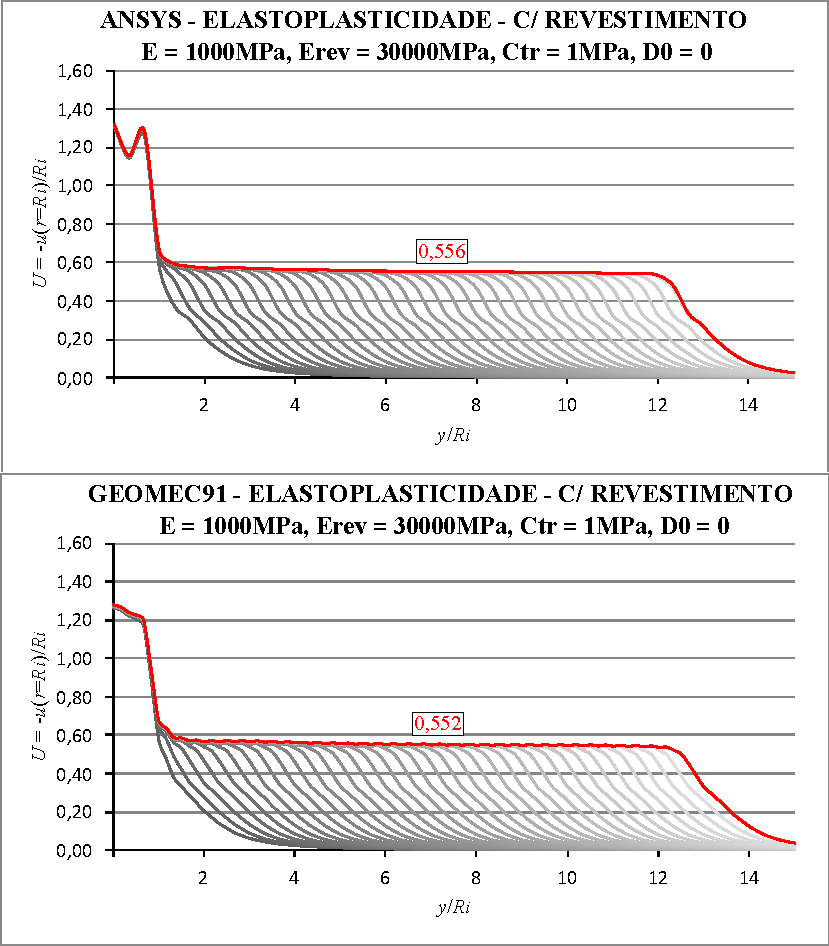
\includegraphics[scale = 1.0]{0713-PLAST-D0-E1000-ER30000-P4-C1.pdf}
	\end{center}
	\caption{\label{PLAST-D0-E1000-ER30000-P4-C1}Verificação solução numérica em elastoplasticidade com revestimento - $E$ = 1000MPa, $E_{rev}$ = 30000MPa, $d0=0$, $c_i=c_p=c_r=\sqrt{3}/2$}
\end{figure}

\subsection{Verificações em viscoplasticidade}

De forma análoga à elasticidade e à elastoplasticidade, o modelo constitutivo acoplado, por ser geral, tem que ser capaz de reproduzir o resultado viscoplástico colocando coesões elevadas na parte elastoplástica.  Considerando $E =$1000MPa, $\nu =$ 0.498MPa, $p_v = p_h = 4$MPa, $c_i=c_p=c_r = \sqrt{3}/2$MPa, $V_p = 5$m/dia tem-se os resultados da \autoref{VISCO-D0-E1000-ER0-P4-C1-V5}. As curvas cinzas abaixo da curva vermelha são os perfis de convergência a cada passo de escavação. A curva vermelha o perfil de convergência da última escavação e colocação do revestimento. A curva azul é o perfil de convergência após os efeitos viscosos cessarem. As curvas cinzas entre a curva vermelha e azul mostram a evolução do perfil de convergências a cada intervalo de tempo.
\begin{figure}[H]
	\begin{center}
		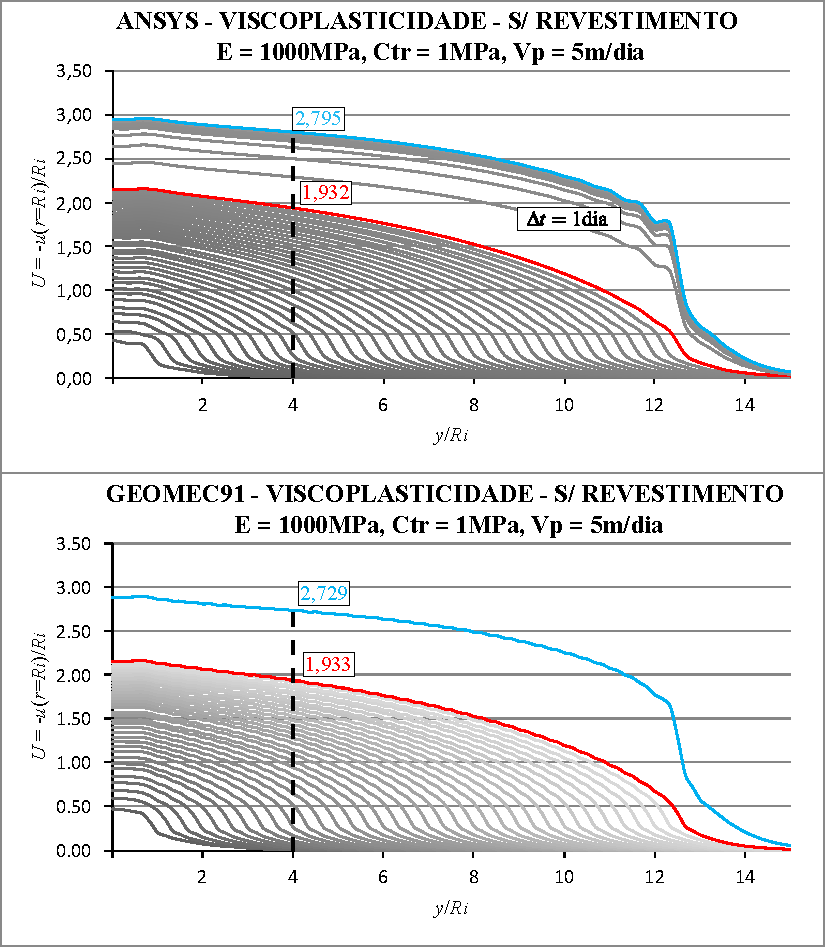
\includegraphics[scale = 1.0]{0714-AXI-D0-E1000-ER0-P4-C1-V5.pdf}
	\end{center}
	\caption{\label{VISCO-D0-E1000-ER0-P4-C1-V5}Verificação solução numérica em elastoplasticidade com revestimento - $E$ = 1000MPa, $c_i=c_p=c_r=\sqrt{3}/2$, $V_p=5$m/dia}
\end{figure}
Como pode-se ver o resultado do GEOMEC91 não apresenta a evolução do perfil de convergências entre o final da construção do túnel e o final dos efeitos viscosos (longo prazo). Outro aspecto é que, para esses parâmetros, não foi atingido um patamar no perfil de convergências, portanto os valores escolhidos para comparação estão na cota $y/R_i$=4. Um aspecto importante a ser notado é que quando se tem apenas viscoplasticidade, sem revestimento, o perfil de convergências no longo prazo tende a se aproximar da solução elastoplástica com os parâmetros do modelo viscoso. Além disso, o perfil de convergências no final da construção do túnel (curto prazo), tende a solução em elasticidade (menores convergências) quando a velocidade de escavação aumenta. A \autoref{VISCO-D0-E1000-ER0-P4-C1-V10} mostra esse aspecto com uma velocidade de 10m/dia.

\begin{figure}[H]
	\begin{center}
		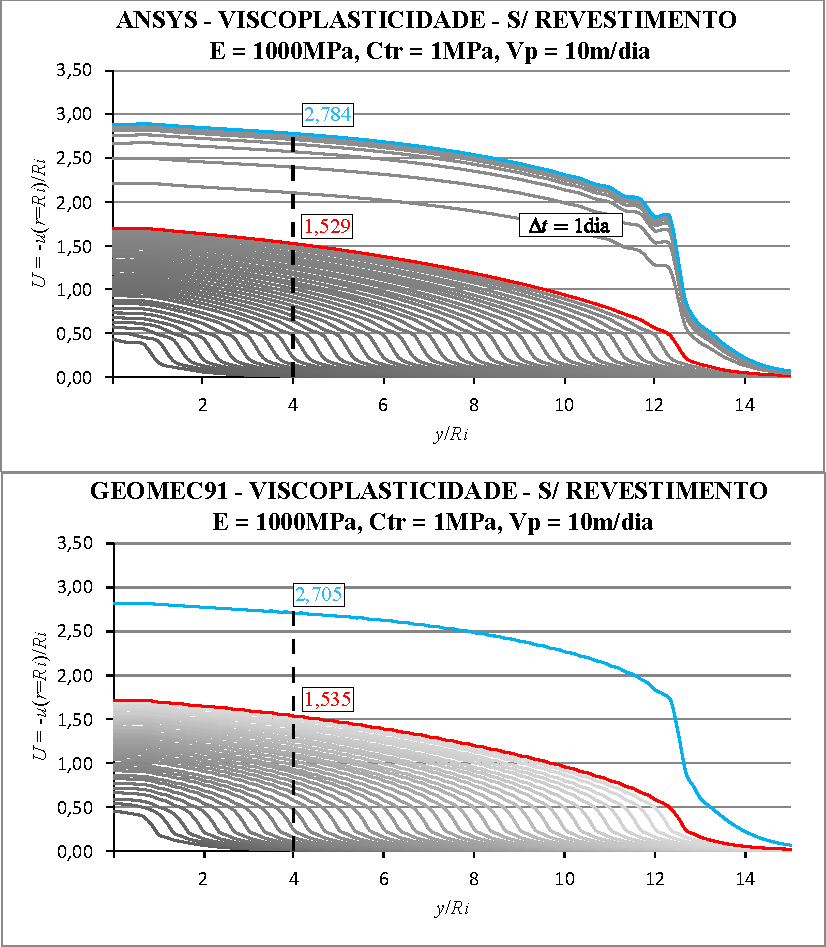
\includegraphics[scale = 1.0]{0715-AXI-D0-E1000-ER0-P4-C1-V10.pdf}
	\end{center}
	\caption{\label{VISCO-D0-E1000-ER0-P4-C1-V10}Verificação solução numérica em elastoplasticidade com revestimento - $E$ = 1000MPa, $c_i=c_p=c_r=\sqrt{3}/2$, $V_p=10$m/dia}
\end{figure}
Como pode-se ver o perfil de convergências no longo prazo não sofreu alteração e o perfil de curto prazo diminuiu suas convergências. O modelo constitutivo acoplado traz diferença justamente nesse aspecto. A convergência no curto prazo será influenciada por eventuais plastificações e a convergência de longo prazo não terá mais esse comportamento de se aproximar da solução elastoplástica com os mesmos valores dos parâmetros viscosos. Haverá uma influência entre os dois comportamentos.

Por fim, para verificar a parte do modelo viscoplástico com revestimento a \autoref{VISCO-D2-E1000-ER3000-P4-C1-V5} apresenta uma comparação considerando um revestimento de $E_{rev}=3000$MPa, $\nu_{rev}=0,3$ colocado com $d_0=2L_p$ afastado da face de escavação.

\begin{figure}[H]
	\begin{center}
		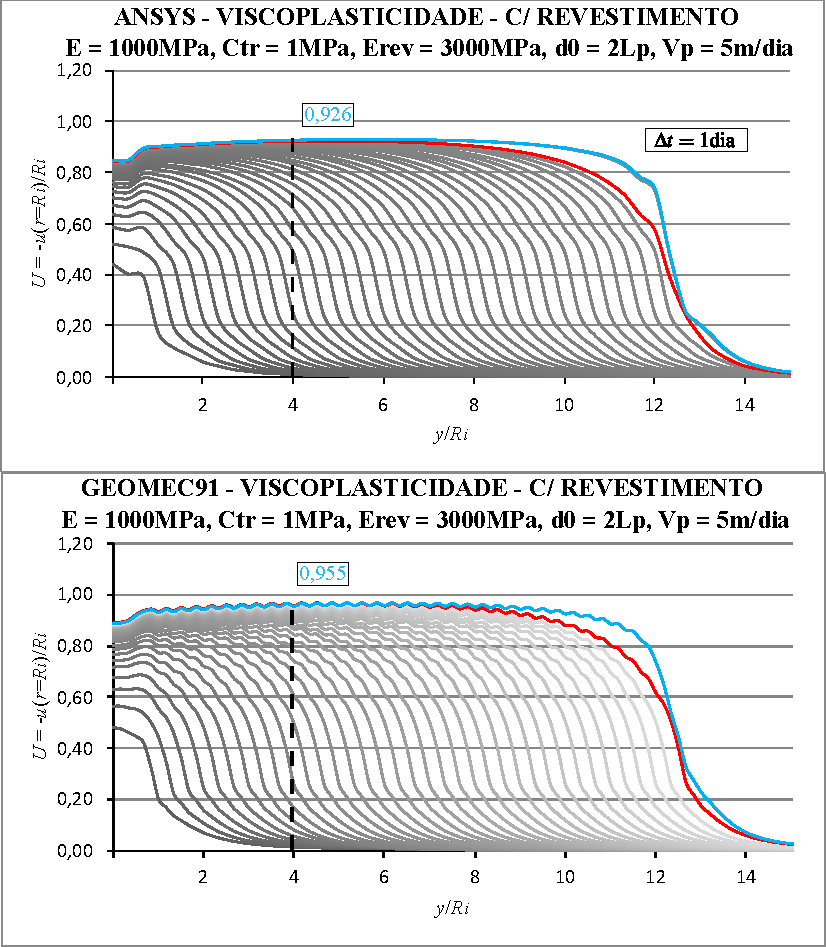
\includegraphics[scale = 1.0]{0716-AXI-D2-E1000-ER3000-P4-C1-V5.pdf}
	\end{center}
	\caption{\label{VISCO-D2-E1000-ER3000-P4-C1-V5}Verificação solução numérica em elastoplasticidade com revestimento - $E$ = 1000MPa, $c_i=c_p=c_r=\sqrt{3}/2$, $E_{rev} = 3000$MPa, $d0=2L_p$, $V_p=5$m/dia}
\end{figure}
Nesse caso, pode-se notar que o revestimento elástico bloqueou a evolução da convergência no longo prazo fazendo com que as deformações de curto (logo após a construção do túnel) e de longo prazo coincidissem. Quando se tem um revestimento viscoso, como o concreto que sofre fluência e retração, esse bloqueio não é tão eficiente. Isso pode ser visto em \citeonline{Quevedo2017}.


\section{Verificação do modelo elastoplástico -viscoplástico com uma solução analítica}

Como exemplo de verificação do algoritmo acoplado implementado é feita a comparação com a solução analítica deduzida por \citeonline[p. 61]{Piepi1995} para um túnel profundo em condições geostáticas-hidrostáticas no interior de um maciço com comportamento elastoplástico-viscoplástico perfeito obedecendo ao critério de Tresca. Essa solução analítica foi escolhida por utilizar o mesmo princípio de associação da \autoref{lei_endurecimento_rousset}, como pode ser visto em \citeonline[p. 35]{Piepi1995}. Contudo, não apresenta a mesma generalidade da solução numérica implementada e possui algumas hipóteses simplificativas, dentre elas, a consideração da mesma superfície de escoamento para plasticidade e viscoplasticidade e vetores de fluxo totalmente associados, ou seja, $\fl^p = \gl^{p} = \fl^{vp} = \gl^{vp}$. Para essa verificação é utilizado o modelo axissimétrico com os seguintes parâmetros: $E=1500$MPa e $2000$MPa, $\nu=0.498$, $c^i=c^p=c^r =4\sqrt{3}/2$MPa, $c^{vp}=3\sqrt{3}/2$MPa, $\eta = 4 \cdot 10^4$dia, $n=1$, $f_0=1$MPa e $p_v=p_h=9$MPa. Esses parâmetros são os mesmos utilizado por \citeonline[p. 131]{Piepi1995} que chegou nas convergências de $U=2,16$ para $E=1500$MPa e $U=1,6$ para $E=2000$MPa.

Como a solução analítica está deduzida para superfície de Tresca e aqui será utilizado a de Drucker-Prager (que se particulariza para von-Mises devido a ausência de ângulo de atrito) foi adotado a relação (\ref{eq:ctr_cvm}) considerando von-Mises inscrito em Tresca nos valores das coesões. A solução analítica obtém o perfil de convergência apenas no longo prazo. Contudo, para mostrar as diferenças entre os modelos, além da solução numérica elastoplástica-viscoplástica (EP-VP), foi feito também a solução considerando cada comportamento separado, ou seja, elástico (E), elastoplástico (EP) e viscoplástico (VP) tanto no final da escavação quanto no longo prazo. Para ver a influência da velocidade de escavação será considerado três velocidades $V_p=0,1; 0,2$ e 10m/dia.

A \autoref{PIEPI-E1500-FINALESCAVACAO} apresenta os resultados no final da escavação. Pode-se notar que os perfis de convergência para o modelo viscoplástico (VP) são intermediários entre o modelo elástico (E) e elastoplástico (EP), sendo que quanto mais rápida a escavação, mais a resposta desse modelo se  aproxima da convergência do maciço em elasticidade. Isso é um resultado esperado, pois quanto maior a velocidade de escavação menos tempo transcorreu para a evolução das deformações viscosas. O modelo elastoplástico-viscoplástico (EP-VP) apresentou a mesma relação com a velocidade (quanto mais rápido menos tempo para as deformações viscosas evoluírem), porém, iniciou suas deformações próximas do perfil de convergências do modelo elastoplástico (EP). Isso ocorre, pois, o maciço atingiu a plastificação durante a escavação. \textbf{Esse é um dos principais objetivos e vantagem desse modelo acoplado}, pois geralmente a escavação induz um comportamento elastoplástico no maciço próximo à abertura e esse efeito não é captado pelos modelos que consideram apenas a viscoplasticidade.

\begin{figure}[H]
	\begin{center}
		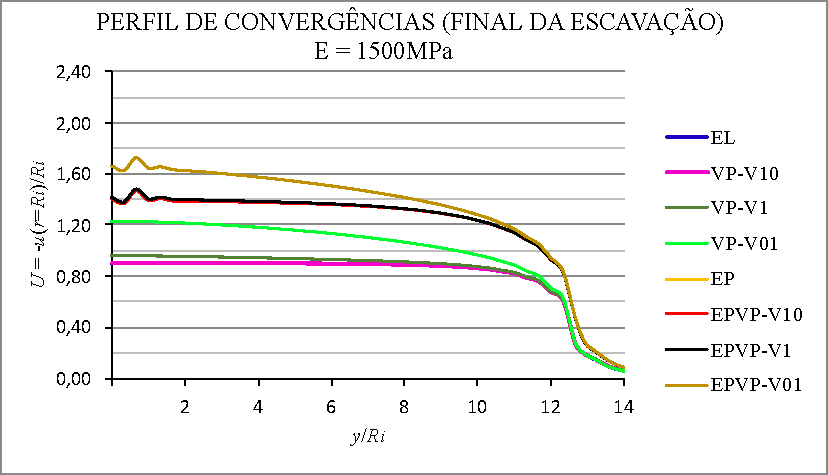
\includegraphics[scale = 1.0]{0717-PIEPI-E1500-FINALESCAVACAO.pdf}
	\end{center}
	\caption{\label{PIEPI-E1500-FINALESCAVACAO}Perfil de convergências no final da escavação para os diversos comportamentos implementados, considerando os parâmetros físicos do maciço de acordo com \citeonline{Piepi1995} com $E=1500$MPa}
\end{figure}

Após o final da escavação, os perfis de convergências dos modelos (VP) e (EP-VP) continuam evoluindo com uma taxa cada vez menor devido a redistribuição de tensões no interior do maciço, até estabilizarem (no longo prazo). A \autoref{PIEPI-E1500-LONGOPRAZO} mostra o perfil de convergência no longo prazo (cerca de 500 dias). Pode-se ver que independente da velocidade de escavação, os perfis de convergêncais viscoplásticos (VP) se estabilizam sobre o perfil da elastoplasticidade (EP). Isso ocorre pois é utilizado a mesma superfície de escoamento em ambos os modelos. Contudo, os perfis do modelo elastoplástico-viscoplástico (EP-VP) encontram a estabilização bem acima do perfil do modelo elastoplástico (EP), o que mostra, mais uma vez a importância da magnitude desse comportamento acoplado. Pode-se ver também que a solução numérica no longo prazo ficou satisfatória com a solução analítica.

\begin{figure}[H]
	\begin{center}
		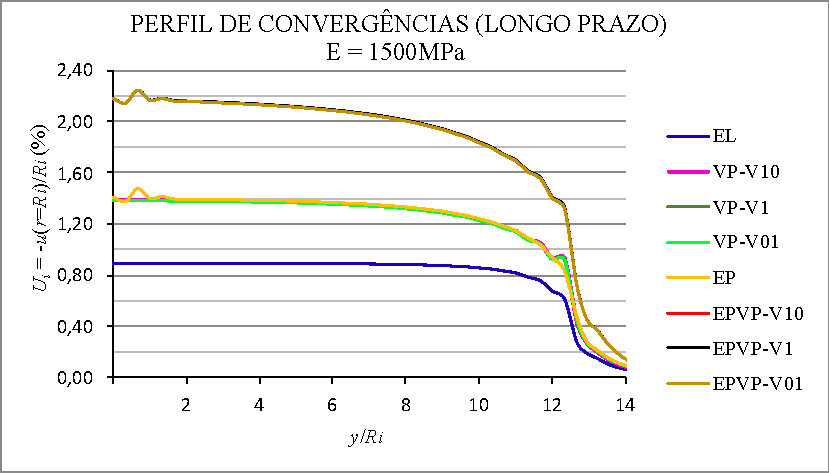
\includegraphics[scale = 1.0]{0718-PIEPI-E1500-LONGOPRAZO.pdf}
	\end{center}
	\caption{\label{PIEPI-E1500-LONGOPRAZO}Perfil de convergências no longo prazo para os diversos comportamentos implementados, considerando os parâmetros físicos do maciço de acordo com \citeonline{Piepi1995} com $E=1500$MPa}
\end{figure}

A \autoref{PIEPI-E2000-FINALESCAVACAO} e \autoref{PIEPI-E2000-LONGOPRAZO} mostram os resultados para $E=2000$MPa. O mesmo raciocínio se aplica nesse caso, porém, como tem maior módulo de elasticidade, os perfis possuem menores convergências.

\begin{figure}[H]
	\begin{center}
		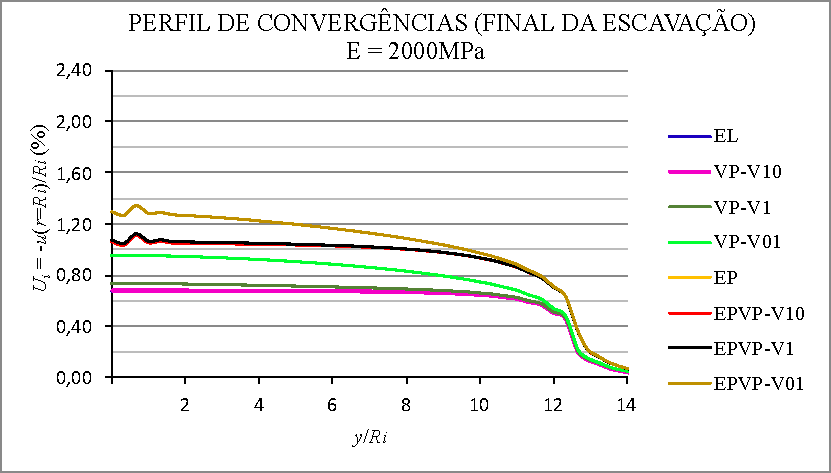
\includegraphics[scale = 1.0]{0719-PIEPI-E2000-FINALESCAVACAO.pdf}
	\end{center}
	\caption{\label{PIEPI-E2000-FINALESCAVACAO}Perfil de convergências no final da escavação para os diversos comportamentos implementados, considerando os parâmetros físicos do maciço de acordo com \citeonline{Piepi1995} com $E=2000$MPa}
\end{figure}

\begin{figure}[H]
	\begin{center}
		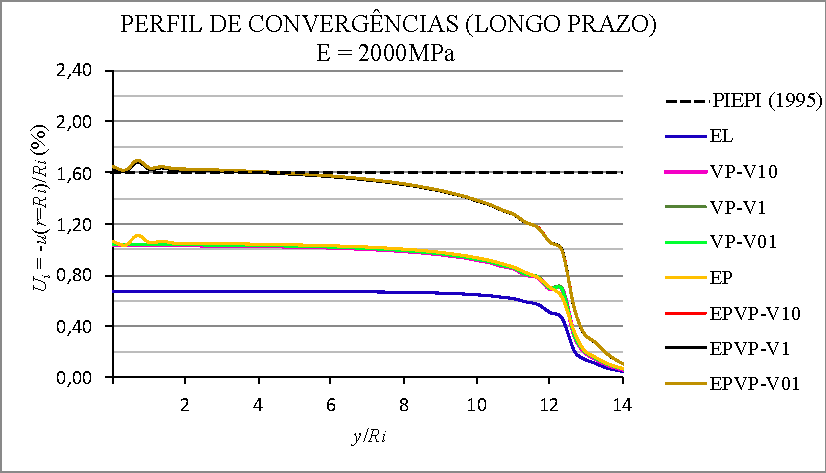
\includegraphics[scale = 1.0]{0720-PIEPI-E2000-LONGOPRAZO.pdf}
	\end{center}
	\caption{\label{PIEPI-E2000-LONGOPRAZO}Perfil de convergências no longo prazo para os diversos comportamentos implementados, considerando os parâmetros físicos do maciço de acordo com \citeonline{Piepi1995} com $E=2000$MPa}
\end{figure}

Os mesmos resultados foram obtidos utilizando o modelo 3D. A \autoref{PIEPI-E1500-CAMPO_DESLOCAMENTO} mostra o campo de deslocamentos no longo prazo para o caso EP-VP com velocidade de escavação $V_p=0,1$m/dia e $E=1500$MPa.

\begin{figure}[H]
	\begin{center}
		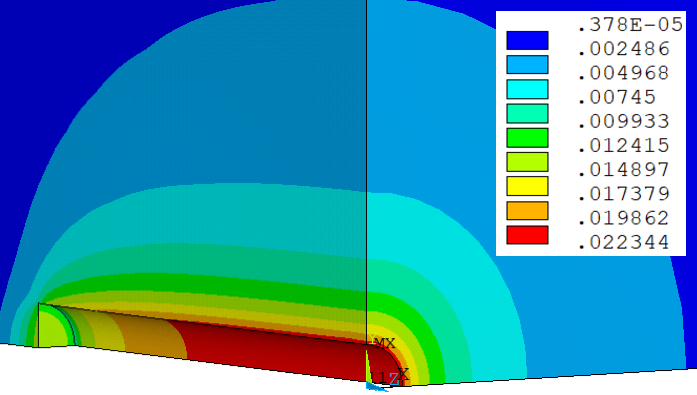
\includegraphics[scale = 1.0]{0721-PIEPI-E1500-CAMPO_DESLOCAMENTO.pdf
		}
	\end{center}
	\caption{\label{PIEPI-E1500-CAMPO_DESLOCAMENTO}Campo de deslocamentos no longo prazo para o caso elastoplástico-viscoplástico com $E=1500$MPa e $V_p=0,1$m/dia}
\end{figure}

A \autoref{PIEPI-E1500-CAMPO_DEFORMACOES} mostra o campo de deformações plásticas e viscosas equivalentes para o mesmo caso.

\begin{figure}[H]
	\begin{center}
		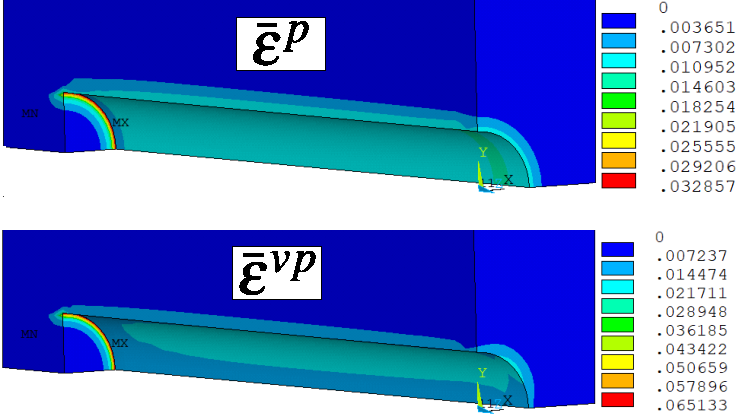
\includegraphics[scale = 1.0]{0722-PIEPI-E1500-CAMPO_DEFORMACOES.pdf
		}
	\end{center}
	\caption{\label{PIEPI-E1500-CAMPO_DEFORMACOES}Campo de deformações plásticas e viscosas no longo prazo para o caso elastoplástico-viscoplástico com $E=1500$MPa e $V_p=0,1$m/dia}
\end{figure}

\section{Análise paramétrica da influência do revestimento}

Nessa seção é apresentada uma análise paramétrica para averiguar a influência do revestimento sobre o perfil de convergência do modelo elastoplástico-viscoplástico. As propriedades do maciço são as mesmas da análise anterior com $E=1500$MPa. É utilizado o modelo em axissimetria, de início sem revestimento e então colocando o revestimento alterando o seu módulo de elasticidade $E_{rev} = 3000$MPa e $E_{rev} = 30000$MPa e a distância não suportada $d0 = 0$ e $d0 = 4L_p$. A \autoref{PARAMETRICO-D0-FINALCONSTRUÇÃO} e \autoref{PARAMETRICO-D0-LONGOPRAZO} mostram os resultados considerando $d_0 = 0$ e a \autoref{PARAMETRICO-D0-LONGOPRAZO} e \autoref{PARAMETRICO-D4-FINALCONSTRUÇÃO} considerando $d_0=4L_p$. A convergência ao equilíbrio é medida em $y/R_i = 6$. 

Comparando o modelo elastoplástico-viscoplástico com o modelo viscoplástico, no final da construção, o primeiro teve, uma convergência 33\% maior sem revestimento. Com revestimento aplicado a $d0=0$ uma convergência entre 17\% e 20\% e para $d0=4L_p$ entre 25\% a 28\% maior. E no longo prazo, o primeiro teve, uma convergência 54\% maior sem revestimento. Com revestimento aplicado a $d0=0$ uma convergência entre 17\% e 23\% e para $d0=4L_p$ entre 26\% a 30\% maior.

\begin{figure}[H]
	\begin{center}
		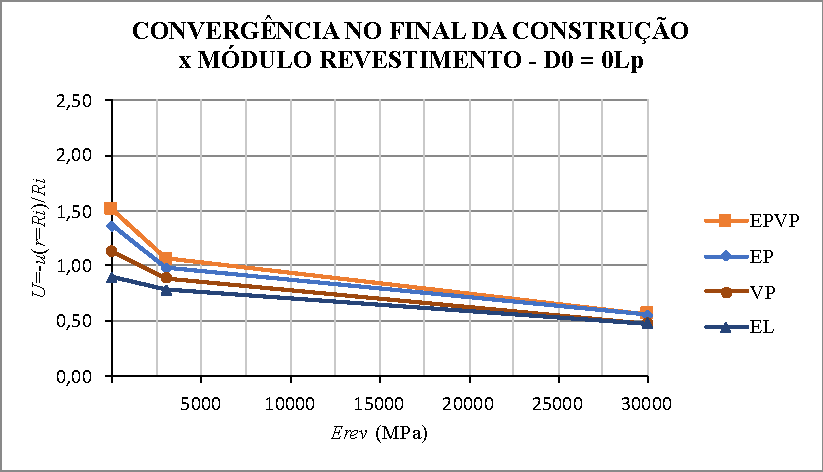
\includegraphics[scale = 1.0]{0723-PARAMETRICO-D0-FINALCONSTRUÇÃO.pdf
		}
	\end{center}
	\caption{\label{PARAMETRICO-D0-FINALCONSTRUÇÃO}Convergência no final da construção \textit{versus} módulo de elasticidade do revestimento para uma distância não revestida $d0=0$}
\end{figure}

\begin{figure}[H]
	\begin{center}
		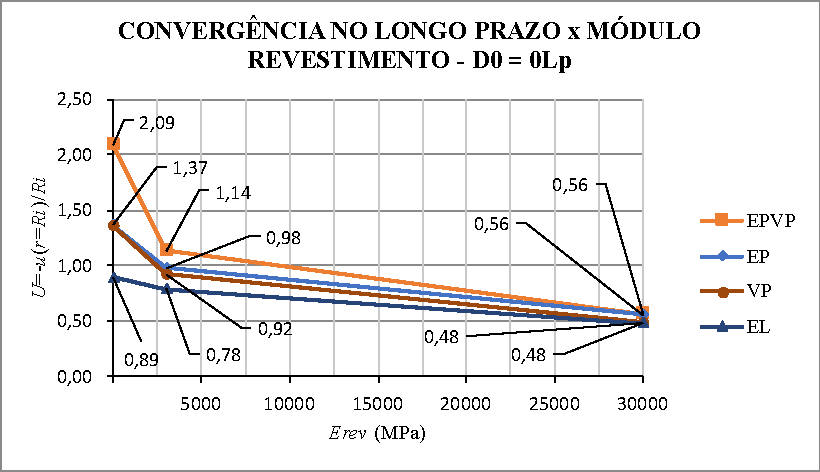
\includegraphics[scale = 1.0]{0724-PARAMETRICO-D0-LONGOPRAZO.pdf
		}
	\end{center}
	\caption{\label{PARAMETRICO-D0-LONGOPRAZO}Convergência no longo prazo \textit{versus} módulo de elasticidade do revestimento para uma distância não revestida $d0=0$}
\end{figure}

\begin{figure}[H]
	\begin{center}
		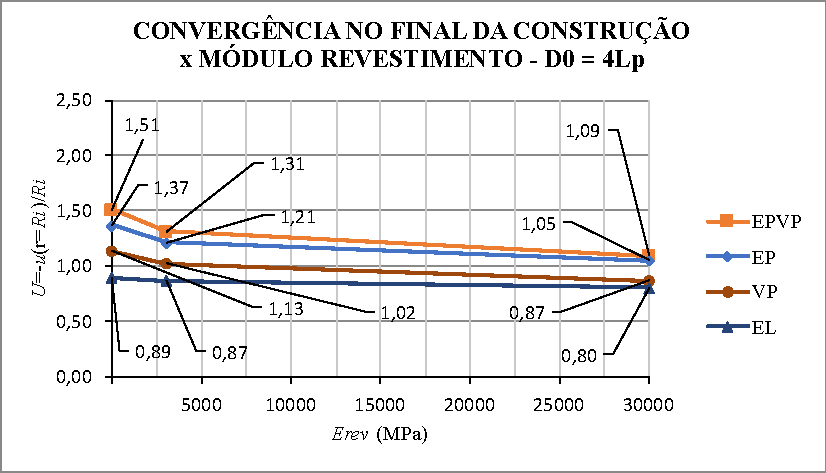
\includegraphics[scale = 1.0]{0725-PARAMETRICO-D4-FINALCONSTRUÇÃO.pdf
		}
	\end{center}
	\caption{\label{PARAMETRICO-D4-FINALCONSTRUÇÃO}Convergência no final da construção \textit{versus} módulo de elasticidade do revestimento para uma distância não revestida $d0=4L_p$}
\end{figure}

\begin{figure}[H]
	\begin{center}
		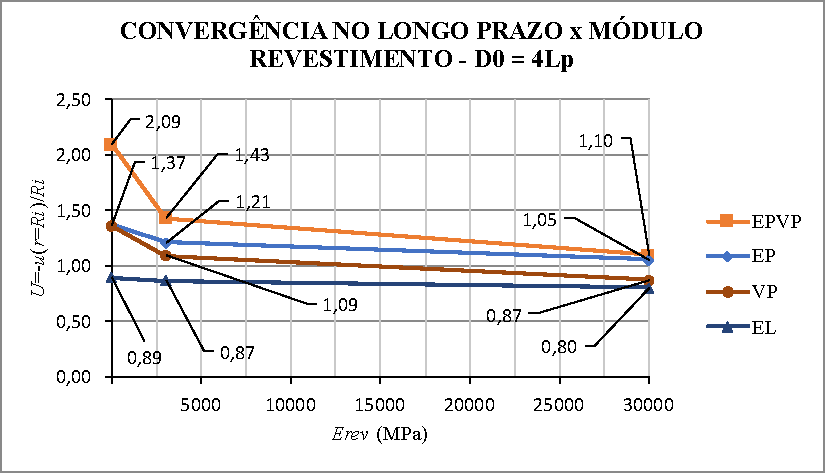
\includegraphics[scale = 1.0]{0726-PARAMETRICO-D4-LONGOPRAZO.pdf
		}
	\end{center}
	\caption{\label{PARAMETRICO-D4-LONGOPRAZO}Convergência no longo prazo \textit{versus} módulo de elasticidade do revestimento para uma distância não revestida $d0=4L_p$}
\end{figure}

\section{Análise da influência de uma seção elíptica}

